\section{Auswertung}
\label{sec:Auswertung}

% % Examples
% \begin{equation}
%   U(t) = a \sin(b t + c) + d
% \end{equation}
%
% \begin{align}
%   a &= \input{build/a.tex} \\
%   b &= \input{build/b.tex} \\
%   c &= \input{build/c.tex} \\
%   d &= \input{build/d.tex} .
% \end{align}
% Die Messdaten und das Ergebnis des Fits sind in Abbildung~\ref{fig:plot} geplottet.
%
% %Tabelle mit Messdaten
% \begin{table}
%   \centering
%   \caption{Messdaten.}
%   \label{tab:data}
%   \sisetup{parse-numbers=false}
%   \begin{tabular}{
% % format 1.3 bedeutet eine Stelle vorm Komma, 3 danach
%     S[table-format=1.3]
%     S[table-format=-1.2]
%     @{${}\pm{}$}
%     S[table-format=1.2]
%     @{\hspace*{3em}\hspace*{\tabcolsep}}
%     S[table-format=1.3]
%     S[table-format=-1.2]
%     @{${}\pm{}$}
%     S[table-format=1.2]
%   }
%     \toprule
%     {$t \:/\: \si{\milli\second}$} & \multicolumn{2}{c}{$U \:/\: \si{\kilo\volt}$\hspace*{3em}} &
%     {$t \:/\: \si{\milli\second}$} & \multicolumn{2}{c}{$U \:/\: \si{\kilo\volt}$} \\
%     \midrule
%     \input{build/table.tex}
%     \bottomrule
%   \end{tabular}
% \end{table}
%
% % Standard Plot
% \begin{figure}
%   \centering
%   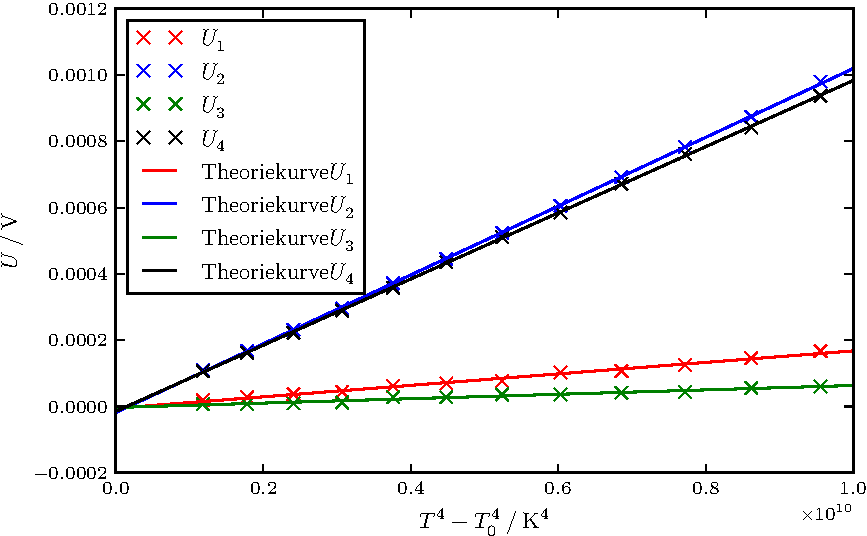
\includegraphics{build/plot.pdf}
%   \caption{Messdaten und Fitergebnis.}
%   \label{fig:plot}
% \end{figure}
%
% 2x2 Plot
% \begin{figure*}
%     \centering
%     \begin{subfigure}[b]{0.475\textwidth}
%         \centering
%         \includegraphics[width=\textwidth]{Abbildungen/Schaltung1.pdf}
%         \caption[]%
%         {{\small Schaltung 1.}}
%         \label{fig:Schaltung1}
%     \end{subfigure}
%     \hfill
%     \begin{subfigure}[b]{0.475\textwidth}
%         \centering
%         \includegraphics[width=\textwidth]{Abbildungen/Schaltung2.pdf}
%         \caption[]%
%         {{\small Schaltung 2.}}
%         \label{fig:Schaltung2}
%     \end{subfigure}
%     \vskip\baselineskip
%     \begin{subfigure}[b]{0.475\textwidth}
%         \centering
%         \includegraphics[width=\textwidth]{Abbildungen/Schaltung4.pdf}    % Zahlen vertauscht ... -.-
%         \caption[]%
%         {{\small Schaltung 3.}}
%         \label{fig:Schaltung3}
%     \end{subfigure}
%     \quad
%     \begin{subfigure}[b]{0.475\textwidth}
%         \centering
%         \includegraphics[width=\textwidth]{Abbildungen/Schaltung3.pdf}
%         \caption[]%
%         {{\small Schaltung 4.}}
%         \label{fig:Schaltung4}
%     \end{subfigure}
%     \caption[]
%     {Ersatzschaltbilder der verschiedenen Teilaufgaben.}
%     \label{fig:Schaltungen}
% \end{figure*}

Um die Grenzspannungen zu bestimmen, wird für fünf Spektrallinien jeweils die Stromstärke in Abhängigkeit von der Gegenspannung gemessen.
Diese Werte werden gewurzelt gegen die Gegenspannung aufgetragen und zugleich wird ein linearer Fit angelegt.
Die Ergebnisse sind in den Abbildungen \ref{plot:1}, \ref{plot:2}, \ref{plot:3}, \ref{plot:4} und \ref{plot:5} zu sehen.
Die Schnittpunkte mit der Spannungsachse nach Ausgleichsrechnungen sind in Tabelle \ref{tab:1} eingetragen.

\begin{figure}
  \centering
  \includegraphics[height=8cm]{build/messung_1.pdf}
  \caption{Messdaten für grünes Licht, $\lambda = \SI{546,07}{\nano\metre}$.}
  \label{plot:1}
\end{figure}

\begin{figure}
  \centering
  \includegraphics[height=8cm]{build/messung_2.pdf}
  \caption{Messdaten für blaugrünes Licht, $\lambda = \SI{491,6}{\nano\metre}$.}
  \label{plot:2}
\end{figure}

\begin{figure}
  \centering
  \includegraphics[height=8cm]{build/messung_3.pdf}
  \caption{Messdaten für violettes Licht, $\lambda = \SI{435,83}{\nano\metre}$.}
  \label{plot:3}
\end{figure}

\begin{figure}
  \centering
  \includegraphics[height=8cm]{build/messung_4.pdf}
  \caption{Messdaten für ultraviolettes Licht, $\lambda = \SI{404,66}{\nano\metre}$.}
  \label{plot:4}
\end{figure}

\begin{figure}
  \centering
  \includegraphics[height=8cm]{build/messung_5.pdf}
  \caption{Messdaten für orangenes Licht, $\lambda = \SI{576,96}{\nano\metre}$.}
  \label{plot:5}
\end{figure}

\begin{table}
    \centering
    \caption{Bestimmung der Schallgeschwindigkeit mittels Durchschallungs-Methode.}
    \label{tab:1}
    \sisetup{parse-numbers=false}
    \begin{tabular}{
	S[table-format=2.2]
	S[table-format=2.1]
	S[table-format=4.2]
	}
	\toprule
	{$h_{\text{zylinder}} \:/\: 10^{-3} \si{\metre}$}		& {$\increment t \:/\: 10^{-6} \si{\second} $}		& 
	{$c_\text{Acryl} \:/\: \si{\metre\per\second} $}		\\ 
	\midrule
    31.30 & 11.5 & 2709.96 \\
61.50 & 22.8 & 2697.37 \\
80.55 & 30.4 & 2645.32 \\

    \bottomrule
    \end{tabular}
    \end{table}


Die Spannungswerte werden nun gegen die jeweilige Frequenz aufgetragen, wobei eine Ausgleichsgerade durch alle Werte gelegt wird.
Das Ergebnis hierzu ist in Abbildung \ref{plot:6} zu begutachten.

\begin{figure}
  \centering
  \includegraphics[height=8cm]{build/messung_6.pdf}
  \caption{Die zuvor berechneten Spannungswerte gegen die jeweilige Frequenz.}
  \label{plot:6}
\end{figure}

Dabei beträgt die Steigung
\begin{align*}
  a = \input{build/a_6.tex},
\end{align*}

welche $\frac{h}{e_0}$ entsprechen sollte, wobei $h$ das Plancksche Wirkungsquantum und $e_0$ die Elementarladung ist.
